\documentclass[twocolumn,tighten]{aastex62}
\turnoffedit 

\shorttitle{Hz-Dyn}
\shortauthors{Xue et al.}


%%%%%%%%%%%%%%%%%%%%%%%%%%%%%
%	load package
%%%%%%%%%%%%%%%%%%%%%%%%%%%%%

\usepackage[us,12hr]{datetime}
\usepackage{graphicx}
\usepackage{gensymb}
\usepackage{listings}
\usepackage{color}
\usepackage{mathrsfs}
\usepackage{natbib}
\usepackage{booktabs}
\usepackage{comment}
\usepackage{morefloats}
\usepackage{sidecap}
\usepackage{grffile}
\usepackage{verbatim}
\usepackage{longtable}
\usepackage{etoolbox}
\usepackage{amsmath}
\usepackage{amssymb}
\usepackage{catchfilebetweentags}
\usepackage{multirow}


\newcommand{\python}{{\sc python}}
\newcommand{\kms}{\mbox{$\rm km\,s^{-1}$}}


\begin{document}

\title{A Uniform Analysis of the Resolved Gas Kinematics in High-Redshift Disk Galaxies}

\author[0000-0001-7689-9305]{Rui Xue}
\affiliation{Department of Physics \& Astronomy, University of Iowa, 203 Van Allen Hall, Iowa City, IA 52242, USA}

\author[0000-0001-9608-6395]{Hai Fu}
\affiliation{Department of Physics \& Astronomy, University of Iowa, 203 Van Allen Hall, Iowa City, IA 52242, USA}

\author[0000-0001-9608-6395]{Friends}
\affiliation{TBD}

\begin{abstract}
TDB
\end{abstract}

\keywords{
galaxies: formation
--- galaxies: high-redshift
--- galaxies: kinematics
}


\section{Introduction}

Our goals:

\begin{itemize}

\item uniform analysis on the gas kinematics of ALMA-resolved high-$z$ disk

\item baryonic/dark matter distribution from RC

\item build a expanding RC database for high-$z$ samples

\end{itemize}

\section{Sample}

ALMA line observations of high-$z$ galaxies are typically done after their redshift are confirmed. 
Some examples of the initial selections: MS SFS (BzK-like), SMGs, or SFRGs (SF radio galaxies).
Blind line surveys do exist.
We began our archival search by looking up objects listed in previous high-$z$ survey papers (as well as some serendipitous objects) in the database.

Originally we planned to focus on MS SFGs, which is not the case anymore.
We can now.

\floattable
\begin{deluxetable*}{cccrccccccccc}[htb!]
\tabletypesize{\small}
\tablecolumns{7} 
\tablecaption{Sample Search (for now)\label{tb:sample}}
\tablewidth{0pt} 
\tablehead{
\multicolumn{1}{c}{Survey}&
\multicolumn{1}{c}{Type}&
\multicolumn{1}{c}{Comments}}
\startdata
\toprule
\citet{Casey:2011aa} & SFRGs & 2 RG southern sources, no ALMA observations \\
\citet{Daddi:2010aa,Daddi:2015aa} & BzK & no southern sources, no ALMA observations \\
\citet{Daddi:2017aa} & X-ray-detected Cluster & no southern sources, 6 sources \\
\citet{Tacconi:2010aa,Tacconi:2013aa,Tacconi:2018aa} & BzK& PHIBSS/PHIBSS2, most are northern sources \\
\citet{Forster-Schreiber:2018aa} & BzK& SINS/zC-SINF, an optical-line-based sample \\
\citet{Jones:2017aa} & various & all [CII] \\
\citet{Pavesi:2018aa} & blind line&	COLDz\\
\bottomrule
\enddata
\tablecomments{
PHIBBS: the $z=1-1.5$ sample is from EGS+CANDELS; the $z\approx2$ sample is from BX/MD. SINS/zC-SINF: from the zCOSMOS and BX/MD.
}
\end{deluxetable*}

\begin{deluxetable*}{cccrccccccccc}[htb!]
\tabletypesize{\small}
\tablecolumns{7} 
\tablecaption{ALMA Sample Compilations\label{tb:sample}}
\tablewidth{0pt} 
\tablehead{
\multicolumn{1}{c}{Object}&
\multicolumn{1}{c}{$\alpha_{\rm J2000}$}&
\multicolumn{1}{c}{$\delta_{\rm J2000}$}&
\multicolumn{1}{c}{$z$ }&
\multicolumn{1}{c}{Program}&
\multicolumn{1}{c}{P.I.} &
\multicolumn{1}{c}{Beam} &
\multicolumn{1}{c}{Lines} &
\multicolumn{1}{c}{Ref.}\\
\multicolumn{1}{c}{}&
\multicolumn{1}{c}{deg}&
\multicolumn{1}{c}{deg}&
\multicolumn{1}{c}{}&
\multicolumn{1}{c}{}&
\multicolumn{1}{c}{}&
\multicolumn{1}{c}{} &
\multicolumn{1}{c}{} &
\multicolumn{1}{c}{} &
\multicolumn{1}{c}{}
}
\startdata
\toprule
COSCLUSTER		&150.2373 &2.3381	&	&2016.1.01155.S	&Wang	&	&	&	1\tablenotemark{a}	\\
BX610			&356.5392 & 12.8221&	&2013.1.00059.S	&Aravena	&	&	&	2,3\tablenotemark{a}	\\
%CosmisEye		&	&	&	&	&	&	&	&	&	\citet{}\\
zc400258			&149.9483 & 1.7386&	&2015.1.00220.S	&Genzel	&	&	&	3\tablenotemark{a}	\\
HZ09			&	&	&	&2012.1.00523.S	&Capak	&	&	&	4\tablenotemark{b}\\
HZ10			&	&	&	&2012.1.00523.S	&Capak	&	&	&	4\tablenotemark{b}\\
J0817+1351		&	&	&	&2015.1.01564.S	&Neeleman&	&	&	4\tablenotemark{b}\\
AzTEC-C159		&	&	&	&2012.1.00978.S	&Karim	&	&	&	4\tablenotemark{b}\\
J1000+0234		&	&	&	&2012.1.00978.S	&Karim	&	&	&	4\tablenotemark{b}\\
J1319+0950		&	&	&	&2012.1.00240.S	&Wang	&	&	&	4\tablenotemark{b}\\
COS0			&	&	&	&2015.1.00607.S	&Riechers	&	&	&	5\tablenotemark{a}\\
\bottomrule
\enddata
\tablecomments{
Reference: 1~\cite{Daddi:2017aa}; 2~\cite{Tacconi:2013aa}; 3~\cite{Forster-Schreiber:2018aa}; 4~\cite{Jones:2017aa}; 5~\cite{Pavesi:2018aa}
$^{\rm a}$ Reference for the Selection
$^{\rm b}$ Reference for the published ALMA data.
}
\end{deluxetable*}


\section{Analysis}

\begin{itemize}
\item for high-resolution study based on the analysis of HXMM01
\item for low-resolution marginally resolved objects, we may try to extract line radial profile and kinematics characteristic using a simplified ``proper'' model.
\item {\bf We can introduce a toy model for the baryonic/DM distribution, which can help regulate the RC shape. The number of free parameters can be largely reduced, and it's possible that we can still extract meaningful information like the DM fraction without measuring or estimating baryonic mass using line luminosity.}
\item Maybe we can do tracer comparisons (if such multi-line tracer exists).
\end{itemize}

\section{Discussion}

\subsection{Comparison among High-$z$ Galaxies (e.g. MS-SFGs vs. SB)}

\citet{Drew:2018aa,Calistro-Rivera:2018aa,Forster-Schreiber:2018aa,ForsterSchreiber:2009hm,Genzel:2017fa,Lang:2017aa,Wisnioski:2015gk,Newman:2013ex,Decarli:2016ab}

\subsection{Comparison with Local Galaxies}

\citet{de-Blok:2008aa,Lelli:2016ab,Erroz-Ferrer:2016aa,Leung:2018aa,Bertemes:2018aa}


\subsection{Tracer-wise}

\citet{Valentino:2018aa,Levy:2018aa}


\subsection{Physics-wise}

\citet{Burkert:2010aa,Davies:2018aa}

\subsection{method-wise}

\citet{Tak:2018aa,Hogg:2018gw}

\clearpage
\appendix

\section{ATLAS}

provide a multi-panel figure for each object:
panel1: x-y mom0 map; panel2: x-v/y-v mom0 map; panel 3: integrated spectrum.

\section{Models of DM/Baryonic Mass Distributions}

For an exponential disk with scale length $r_{\rm d}$, we have
\begin{equation}
v_{\rm rot}^2=v_0^2-2 \sigma^2 \left(\frac{r}{r_{\rm d}} \right),
\end{equation}
in which 
\begin{eqnarray}
v_0^2(r) & = & v_{\rm disk}^2(r) + v_{\rm DM}^2(r') \\
r' & = & r \left[ 1+\frac{r \times v_{\rm disk}^2(r)}{r' \times v_{\rm DM}^2(r')} \right] .
\end{eqnarray}
\begin{equation}
v_{\rm disk}^2(r) = 4 \pi G \Sigma_0 \ r_{\rm d} y^2 [I_0(y) K_0(y) - I_1(y) K_1(y)]
\end{equation}
and 
\begin{equation}
v_{\rm DM}^2(r')=V_{200}^2 \left( \frac{r_{200}}{r'} \right) \frac{ln(1+r'/r_{\rm s})-(r'/r_{\rm s})/(1+r'/r_{\rm s})}{ln(1+c)-c/(1+c)}.
\end{equation}
The scale radius
is related to the virial radius $r_{200}$ via $r_s=r_{200}/c$
where $c$ is the halo concentration parameter. 
$\Sigma_0$ is determined by the total disk mass 
$M_d = m_d \times M_{200}$ with $m_d$ the disk mass fraction of the galaxy (the ratio?)

\begin{equation}
\Sigma_0 = m_d \frac{M_{200}}{2 \pi r_{d}^2} .
\end{equation}

Free parameters set: $m_{\rm vir}$, $z$, $m_{\rm ratio}$, $r_{\rm mdisk}$,$v_{\rm sigma}$, inc, $r_{\rm line}$,$r_{\rm disk}$.

\section{notes on coding}

We may use existing Python modules so the focus of this project will become data compilation, and model-data comparison. We can still publish the code which glues different pieces together.
However, as a bottom line we will check if the results from the borrowed codes pass some basic sanity check and we need to gain enough understanding on their implementations.

\begin{itemize}

\item We can borrow KinMSpy\footnote{\url{http://www.astro.cardiff.ac.uk/pub/Tim.Davis/code.php}} for generating cubes. The clear advantage is that it's purely based on Python/Astropy. Some minor changes may be need for our purpose.

\item As for the DM profiles, various existing Python library can be borrow: Colossus\footnote{\url{http://www.benediktdiemer.com/code/colossus}}, Halotools \citep{Hearin:2017aa}, gammapy\footnote{\url{https://docs.gammapy.org/dev/astro/darkmatter/index.html}},
galpy \footnote{\url{https://galpy.readthedocs.io/en/v1.4.0}}.
Some related reading: \citet{Diemer:2017aa,Robotham:2018aa,Mead:2015aa}

\item UVMCMCFIT \footnote{\url{https://github.com/sbussmann/uvmcmcfit}}

\item UVMULTIFIT  \footnote{\url{https://www.oso.nordic-alma.se/software-tools.php}}


\end{itemize}


\begin{figure}%[h!]
\centering
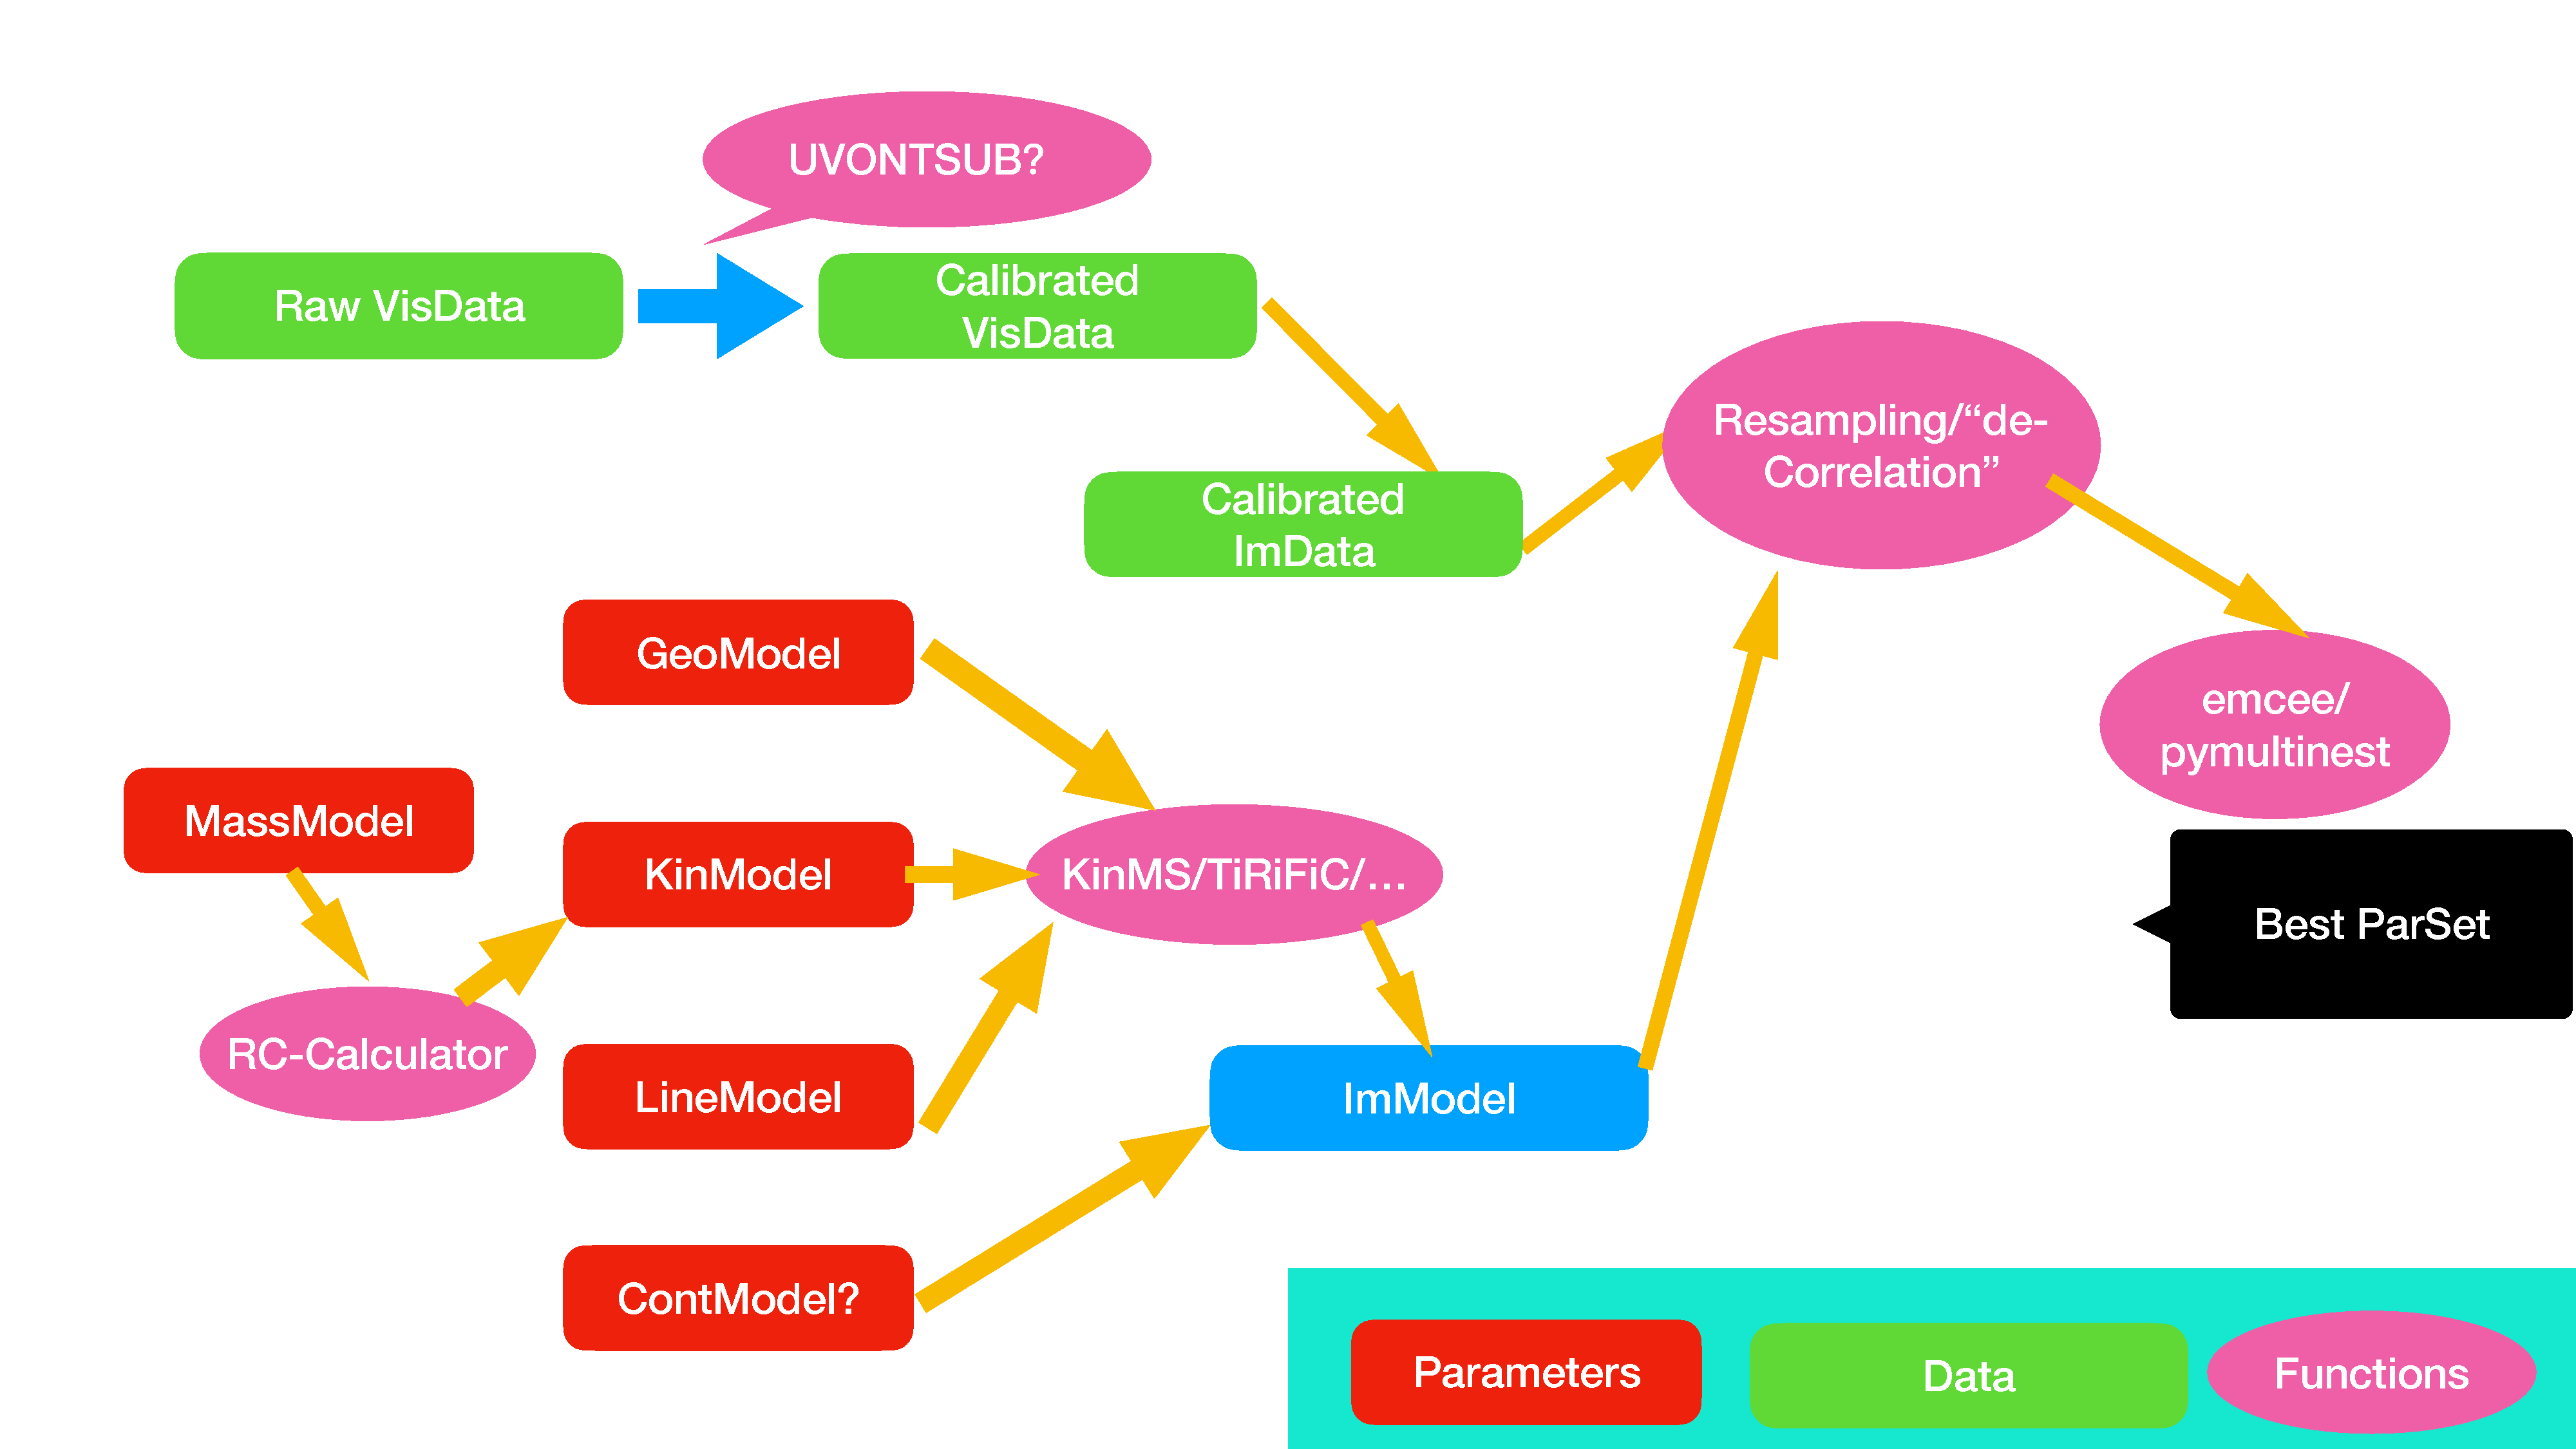
\includegraphics[width=0.80\textwidth]{figures/pipeline-workflow-im.pdf}
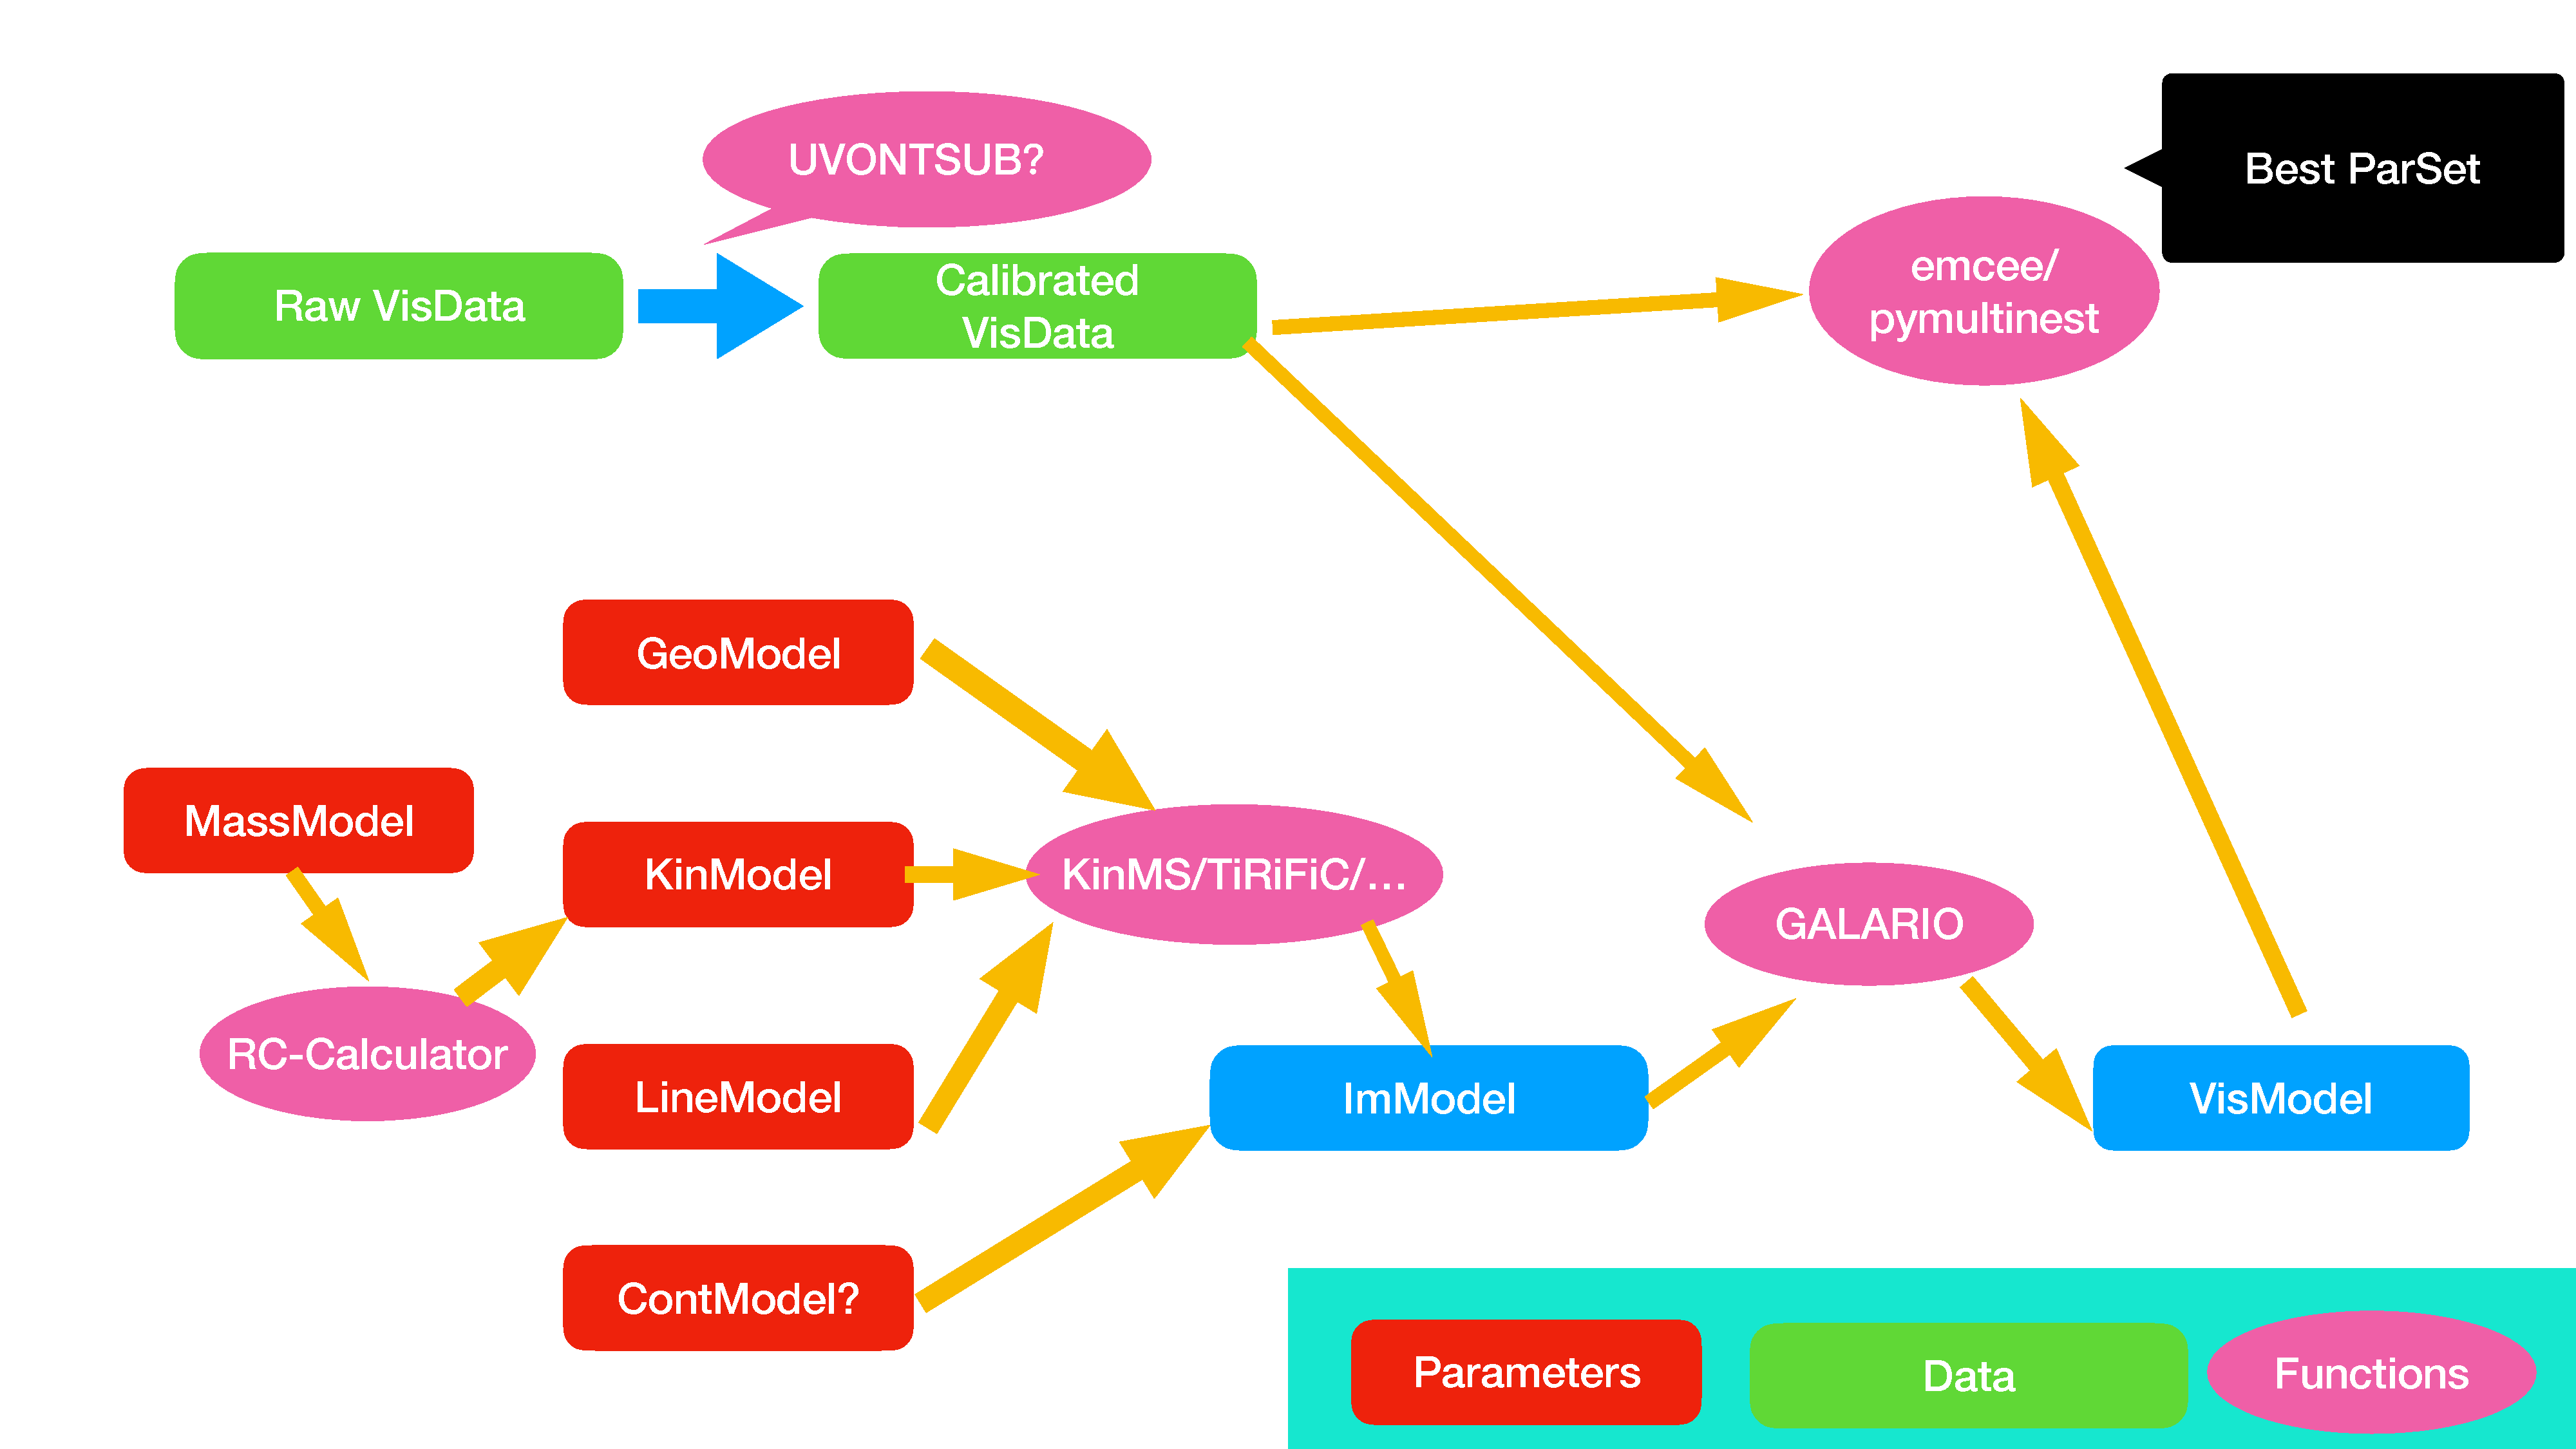
\includegraphics[width=0.80\textwidth]{figures/pipeline-workflow-vis.pdf}
\caption{code structure/workflow: xy-version/uv-version
\label{fig:spec}
}
\end{figure}

\begin{figure}%[h!]
\centering
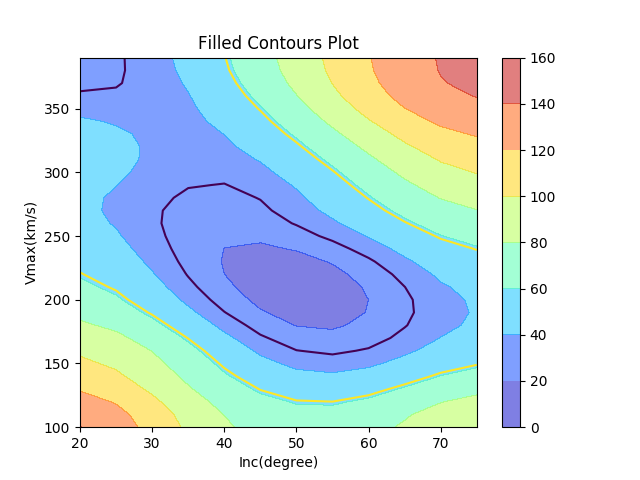
\includegraphics[width=0.48\textwidth]{figures/chisq_test.png}
\caption{$\chi^2$ as a function of the galactic disk inclination and $v_{\rm max}$. The value is directly derived from comparisons of the visibility data and model. 
The intrinsic model is a rotating disk with $v_{\rm max}=210$\,\kms and an inclination of $i=50\degree$.
\label{fig:spec}
}
\end{figure}

\section{HXMM01 test}

This paper makes use of the following ALMA data: ADS/JAO.ALMA#2017.1.01045.S. ALMA is a partnership of ESO (representing its member states), NSF (USA) and NINS (Japan), together with NRC (Canada), NSC and ASIAA (Taiwan), and KASI (Republic of Korea), in cooperation with the Republic of Chile. The Joint ALMA Observatory is operated by ESO, AUI/NRAO and NAOJ.The National Radio Astronomy Observatory is a facility of the National Science Foundation operated under cooperative agreement by Associated Universities, Inc

\bibliography{ms-hzdyn}

\end{document}
